\documentclass[runningheads,a4paper]{llncs}

\usepackage{amssymb}
\setcounter{tocdepth}{3}
\usepackage{graphicx}
\usepackage{tikz}
\usepackage[T1]{fontenc}
\usepackage[scaled]{beramono}
\usepackage{listings}
\usepackage{color}
\usetikzlibrary{arrows,chains,positioning,scopes,quotes,calc}
\usepackage{float}

\newcommand{\keywords}[1]{\par\addvspace\baselineskip
\noindent\keywordname\endspace\ignorespaces#1}
\pagestyle{plain}
\setlength\parindent{0pt}

\definecolor{mygreen}{RGB}{28,172,0} % color values Red, Green, Blue
\definecolor{mylilas}{RGB}{170,55,241}

\newcommand*{\StrikeThruDistance}{0.15cm}%
\newcommand*{\StrikeThru}{\StrikeThruDistance,\StrikeThruDistance}%

\tikzset{strike thru arrow/.style={
    decoration={markings, mark=at position 0.5 with {
        \draw [blue, thick,-] 
            ++ (-\StrikeThruDistance,-\StrikeThruDistance) 
            -- ( \StrikeThruDistance, \StrikeThruDistance);}
    },
    postaction={decorate},
}}

\lstset{
  language=Python,
  showstringspaces=false,
  formfeed=\newpage,
  tabsize=4,
  commentstyle=\itshape,
  basicstyle=\ttfamily,
  morekeywords={models, lambda, forms}
}

\begin{document}
\def \SystemName {Worlds} % Lol because this shit probably will change.

\mainmatter  % start of an individual contribution

% This needs some work, big time.
\title{\SystemName: A distributed MMO}

\author{Ryan Walker\\
				ryan.cjw@gmail.com}

\institute{} %Merp

\maketitle
%% Scrum area
%% TODO:
% Not controlled by centralized organization.
% How/Where are the actual files hosted? Client Files??
%	-> How are these fetched?

\begin{abstract}
% A protocol defining how anyone can contribute to an unbounded universe could allow the flexibility to organically grow an MMO faster than any proprietary system. This paper overviews a protocol that enables developers to bolt their game into in common universe. 
This paper overviews a protocol that aims to manage the large scale economic components of a distributed MMO. Following the implementation of the Worlds protocol it becomes possible to fairly scale a game universe based on games developed by completely independent parties. 
\end{abstract}

\section{Worlds}
\subsection{Introduction}
For an open software ecosystem to grow organically there should be outlets for contribution. In the context of a massively multiplayer online game the outlets become more complicated then a simple code repository. Fair game mechanics are built on a fragile ecosystem that have negative consequences if managed improperly. Forming consensus on a network is trivially done with conventional methods. A server maintains a secure connection with a player who pipes actions to the server. The server then provides ground truth for the network. Our model replaces a centralized organization with a smart contract which forms consensus and balances the economics of the universe. The user experience is designed by anyone who wishes to contribute.

\subsection{Overview}
A world, defined as $w_k$, is a node that designs a user experience and hosts players. Worlds provide the game client which the players interact with. In addition they govern their world and create the elements that make it unique. A world can have up to four adjacent worlds determined by itself. This forms a network, which allows players to explore and move common items (\ref{items}), experience (\ref{exp}) and currency (\ref{money}) between worlds.

\begin{small}
\tikzset{myblock/.style = {rectangle, draw, minimum height=1cm, minimum width=3cm}}
\begin{center}
\begin{tikzpicture}
\label{Hello}
\node(WE)[myblock]{\begin{tabular}{c}Worlds Engine \\ {\scriptsize Worlds.js} \\\end{tabular}};
\node (WS)[myblock,above of=WE, yshift=1cm]{\begin{tabular}{c}Worlds Engine\\ {\scriptsize Worlds.js} \\\end{tabular}};
\node (WC)[myblock,left of=WE, xshift=-3cm]{\begin{tabular}{c}Game Client \\ {\scriptsize \textit{From game Dev}} \\\end{tabular}};
\node (SE)[myblock,left of=WS, xshift=-3cm]{\begin{tabular}{c}Server Engine \\ {\scriptsize \textit{From game Dev}} \\\end{tabular}};
\node (WSC)[myblock,right of=WS, xshift=3cm, yshift=-1cm]{\begin{tabular}{c}Smart Contract (\ref{WSC}) \\ {\scriptsize \textit{On Chain}} \\\end{tabular}};

\draw [dashed] (-6,1) -- (2,1);
\draw [dashed] (2,2.5) -- (2,-0.5);

\node [left of=SE, xshift=-1cm]{\begin{tabular}{c}Server\\Side\end{tabular}};
\node [left of=WC, xshift=-1cm]{\begin{tabular}{c}Client\\Side\end{tabular}};
\node [below of=WSC]{Blockchain};

% \draw[<->] ($(WE.north east)!0.5!(WE.north west)$) --  ($(WS.south east)!0.5!(WS.south west)$);
\draw[<->] (WC) -- (WE);
\draw[<->] (SE) -- (WS);
\draw[<->] (SE) -- (WC);
\draw[<->] ($(WSC.north west)!0.25!(WSC.south west)$) --  ($(WS.north east)!0.5!(WS.south east)$);
\draw[<->] ($(WSC.north west)!0.75!(WSC.south west)$) --  ($(WE.north east)!0.5!(WE.south east)$);
% TODO: Change the arrow heads. 
\end{tikzpicture}
\end{center}
\end{small}
The worlds engine is an application that manages the elements that are common throughout all worlds, such as player keys, hashing+signing and fetching the files required to run the Game Client. The world designer has full creative freedom over the game client and server engine. This enables the highest flexibility and the most unique universe. It is possible for clusters of worlds to share a single game client, yet design their own experience. Conversely, adjacent worlds might have completely different game clients, where players might move from a text based MUD into a fully 3D world. The worlds client takes care of fetching the executable game client from the worlds server.

\section{Worlds Smart Contact (WSC)}
\label{WSC}
The worlds smart contract is used to form consensus among the network. It contains functions and data elements that are used as various forms of proof that require interoperability between worlds. An appropriate blockchain with the following requirements has not yet been selected, it must satisfy the following requirements. 

\begin{itemize}
\item{Low networks fees}
\item{Fast transactions for in game purchases}
\item{Decent data capacity to hold merkle proofs}
\end{itemize}

\section{Actions}
Actions are defined as anything a node can do to effect the network. Messages and data packages are to be considered actions in this context.

\subsection{Direct Action}
A direct action is any action that is travels between the Server Engine and the Game Client. These actions have the lowest latency. An example of an action like this might be the Server engine telling the Game Client of some in game event. Before there can be communication like this the there needs to be a symmetric key exchange. 

\subsection{Proof Action}
A proof action are actions that require the use of private keys for signing, but then relay the signed package from the Game Client to the Server Engine. For nodes that require higher security it is possible to hold the Worlds Engine offline therefor keeping their keys offline. 

\subsection{Contract Action}
Contract actions are any actions that communicate with the Worlds Smart Contract. They can be issued from the Worlds Engine directly, or the Game Client can pipe action requests into the worlds engine. 

\section{Experience}
\label{exp}
Experience is distributed to players using experience packages. These are of the form (Figure \ref{exppkg}). When a player is to received experience this package is hashed, signed and sent to the \textit{Worlds Smart Contract} (\ref{WSC})(WSC). The world must stake some WOR in order to grant experience. Experience is distributed like items, although it is not transferable. It is possible for experience to be liquidated back into WOR by the players. Worlds determine the effect of player experience, typically the more WOR that is staked the larger the effect can be. It is possible for players to stake their own WOR and buy experience. However this experience is stamped with the public key of the issuer and it's possible that worlds might not accept this during the worlds transfer. 


\begin{figure}[H]
\centering
\caption{Experience Package - Sword Fighting}
\label{exppkg}
\begin{lstlisting}
ExpClass = 'SwordFighting'
ExpHash = hash(ExpClass);
PlayerPublic = 0x5d7ac22131ad370e59fddb5f6079a354dbdd2dd9
WorldPublic = 0xb1abdaf3ab936c99f5fd518122cf7d5b811a1a30
IssueTime = UnixTime #Time of Issue
Stake = 0.1WOR
\end{lstlisting}
\end{figure}

\subsection{Receiving Experience} 
In the interest is keeping latency low and conserving space onchain, experience is distributed to players when they leave the world. Although players may use gained experience immediately in their current world.

\section{Items} 
\label{items}
Items can be introduced by any node on the network. To spawn an item the item package, defined as $i$, must be signed by the node and submitted to the \textit{worlds smart contract} to prove ownership and lock the funds associated with the item. The smart contract verifies that the WorldPublic field is the public key of the node issuing the item, assigns current unix time and then moves the WOR into the smart contract from the issuers account. Worlds have the option to credit or discredit certain items based on the WorldPublic field.  It is possible for items to be liquidated back into WOR by calling a function on the WSC. As only the hash of the item package is kept on-chain players are required to keep the entire item package.

\begin{figure}[H]
\centering
\label{itempkg}
\caption{Item Package $i$ - Wood}
\begin{lstlisting}
ItemName = 'Wood'
ItemClass = 'Material'
OwnerPublic = 0x5d7ac22131ad370e59fddb5f6079a354dbdd2dd9
PreviousOwnerPublic = 0xgf7dsa7ejdb5370e59fddb5f6079a354ugf84bdv
WorldPublic = 0xb1abdaf3ab936c99f5fd518122cf7d5b811a1a30
UnixTimeGen = # Time the item was created
UnixTimeTX = # Time the item was last transmitted
Stake = 1WOR
ItemHash = hash(ItemName | ... | Stake);
\end{lstlisting}
\end{figure}

\subsection{Item Transfers}
By calling the TxItem(ItemHash, PlayerPublic) function on the WSC it is possible to transfer items to other players.

\subsection{Staked WOR}
In order to have a balanced economy the monetary system needs to be net zero (\ref{money}). The same holds true for experience and items, this balance is achieved by staking WOR into items and EXP. Without this mechanic worlds would be able to create as much wealth as they want, resulting in over powered items and EXP. 

\subsection{Forging}
\label{Forging}
It is possible to forge items by combining multiple items, thus forming a derivative item. In literal sense the act of forging it to call the function \textit{ForgeItem(Item1, Item2, ...)} on the WSC. This will then make a derivative item which is shown in Figure \ref{ForgedItem}. It is up to the worlds to decide on the item names and item classes of these subitems. As an example, a player may forge a sword by combining metal, fabric and a sharpening stone. As long at the world recognizes that the ForgeHash of the item do in fact form a sword, then the player has crafted a sword for use in these worlds. The power of the sword would be proportional to the amount of stakes WOR in all the items that were used to craft the sword. Once items are forged into something they can no longer be used for anything else. It is possible to unforge an item.

\begin{figure}[H]
\centering
\caption{Forged Item $i_f$}
\label{ForgedItem}
\begin{lstlisting}[escapeinside={(*}{*)}]
ForgeHash = hash((*$i_0[ItemName] |  i_0[ItemClass] | ... | i_n[ItemName] | i_n[ItemClass]$*))
PlayerPublic = 0x5d7ac22131ad370e59fddb5f6079a354dbdd2dd9
WorldPublic[0 .. n] = # Public Key of all the worlds that issued the sub items
ItemHash[0 .. n] = # Item hashes of items in the forge
UnixTimeGen = # Time the item was created
UnixTimeTX = # Time the item was last transmitted
Stake = sum(ParentItemStake)
ItemHash = hash(ForgeHash | ... | Stake);
\end{lstlisting}
\end{figure}

\subsection{Using Items}
In order reduce the latency of item usage, certain actions must be taken off-chain. Please see the section \ref{Staking} for more information on this.

\section{Currency (WOR)}
\label{money}
A common currency between worlds will be used for staking and integration into the platform. To prevent abuse this currency must be zero sum, meaning worlds cannot generate it and it must start with a fixed supply. Ideally it is tracked through an existing blockchain. Worlds can introduce mechanics for generating revenue, like entrance fees, subscriptions, purchasing items, or keeping players items upon a death. Please read more in section \ref{MakeMoney}.

\section{Transport}
To prevent players from playing on multiple worlds concurrently a player location is kept on the worlds smart contract. This location is the public key of the world that the player currently resides. In order for this to be valid it must be signed by the player and the world the player resides in. If a player wishes to travel to a world... 

\begin{itemize}
\item{The player must send a signed entry request to the world.}
\item{If the world only allows travel from adjacent worlds, the player must reside in an adjacent world.}
\item{The player provides proof of items and experience.}
\item{The world might check the public key stamped the items/exp to ensure they are from creditable sources.}
\item{Items or experience are staked if required to be.}
\item{Player is granted access, WSC is updated with player location.}
\end{itemize}

\section{World Incentivisation}
\label{MakeMoney}
If worlds want to distribute items or experience they must stake some WOR into items. As WOR has monetary value worlds need a way to generate some revenue. In order for a world to profit, the sum of all revenue generation methods must be less their their distributed items. Some revenue strategies are similar to existing games, some are completely new. 

\subsection{Staking}
\label{Staking}
Some worlds may require you to stake some experience, items or WOR before entering. This is effectively temporarily moving these into possession of the world. If the player is to die, the staked things will fall under ownership of the world. The world then has the option to...

\begin{itemize}
\item{Redistribute the items among other player, skimming some fee of the top.}
\item{Liquidate all the items for WOR.}
\item{Give all the items, or some of the items, back to the player.}
\end{itemize}

\subsection{Fees}
Just like conventional games, it is possible the worlds might charge an entrance fees. These could be one time or reoccurring. This would be transparent as the player moves about worlds. Ideally the fees would be built into the lore of the game.

\subsection{In Game Purchases}
Worlds might wish to sell items for WOR, this is a grey area as it can be considered pay-to-win. This may be  moderated by the entire ecosystem as worlds have the option to deny items that are issued by certain worlds, this is spoken more to in section \ref{Pay2Win}.\\

Static items are assets that may not transcend worlds, an example being virtual land or housing. These are provided solely by the world of issuance and the value is determined by that world. It is possible they may be kept in the WSC with a staked value of 0 WOR. As worlds are not required to stake WOR against these assets they may profit from selling them for WOR. Items of this class might prove to be an alternate revenue stream.

\section{Outstanding Issues}
\subsection{Malicious Worlds}
Players may be required to stake items, WOR or EXP to enter a world (\ref{Staking}). As the universe grows, worlds may be required to manage lots of wealth, which opens the possibility of an exit scam or hacking.

\subsection{Neighbor Conflict}
Depending on the topology of worlds there may be neighbor conflicts. In the grid model, Figure \ref{GRID}, $w_5$ may wish to be adjacent to $w_2$ but not next to $w_4$. 

\begin{figure}
\centering
\caption{GRID}
\label{GRID}
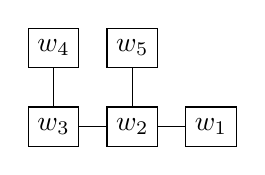
\begin{tikzpicture}
\node[shape=rectangle,draw=black, minimum height=0.5cm, minimum width=0.5cm] (w1) at (0,0) {$w_1$};
\node[shape=rectangle,draw=black, minimum height=0.5cm, minimum width=0.5cm, left of=w1] (w2) {$w_2$};
\node[shape=rectangle,draw=black, minimum height=0.5cm, minimum width=0.5cm, left of=w2] (w3) {$w_3$};
\node[shape=rectangle,draw=black, minimum height=0.5cm, minimum width=0.5cm, above of=w3] (w4) {$w_4$};
\node[shape=rectangle,draw=black, minimum height=0.5cm, minimum width=0.5cm, above of=w2] (w5) {$w_5$};

\draw [-] (w1) -- (w2);
\draw [-] (w2) -- (w3);
\draw [-] (w3) -- (w4);
\draw [-] (w2) -- (w5);
\end{tikzpicture}
\end{figure}

Using a network, Figure \ref{Graph} it's possible to treat the worlds like nodes on a graph. This allows four neighboring connections on every node. How this effects the physical universe is yet to be determined.

\begin{figure}
\centering
\caption{DAG}
\label{Graph}
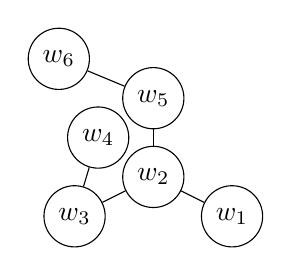
\begin{tikzpicture}
\node[shape=circle,draw=black] (w1) at (-0.3cm,0.1cm) {$w_1$};
\node[shape=circle,draw=black, left of=w1, yshift=0.5cm] (w2) {$w_2$};
\node[shape=circle,draw=black, left of=w2, yshift=-0.5cm] (w3) {$w_3$};
\node[shape=circle,draw=black, above of=w3, xshift=0.3cm] (w4) {$w_4$};
\node[shape=circle,draw=black, above of=w2] (w5) {$w_5$};
\node[shape=circle,draw=black, left of=w5, xshift=-0.2cm, yshift=0.5cm] (w6) {$w_6$};

\draw [-] (w1) -- (w2);
\draw [-] (w2) -- (w3);
\draw [-] (w3) -- (w4);
\draw [-] (w2) -- (w5);
\draw [-] (w5) -- (w6);
\end{tikzpicture}
\end{figure}

\subsection{Developers}
With the initial implementation of the engine there will not be many worlds at first. It will take time for the universe to manifest itself as something massive. It is possible this will never happen due to a lack of developer interest.

\subsection{Blockchain Technology}
We are keeping our eyes open for a suitable blockchain for developing the smart contract. But the space requirements are high, ideally players can bring their own blockchain storage to the party, meaning players pay a small amount for each item they wish to keep. 

\subsection{Unification}
Worlds may have issues forming consensus on forged items (\ref{Forging}). The derivative hash will be the same if all of the items that go into the forge are the same from forge to forge. Although the resultant item of the forge can be controversial. It is possible that worlds can use item translations (\ref{ItemTranslations}, these can be used to funnel many items into a single for use in the world.

\subsection{Congruent Worlds}
As it is possible for each world to have their own client the game may suffer from a disconnect, as players move from world to world and the engine fetches new clients for each world the universe may seem to be disconnected. This may be either positive or negative based on the player. After the development of the Worlds Engine and smart contract, we are confident that there will be clusters of worlds that use the same client for players that want more fluid game play.

\end{document}

\section{Engine Mechanics} 
The mechanics below are simply suggestions. As the engine is completely open, worlds are free to impose whatever mechanics they wish. Worlds with drastically different game mechanics will probably not be bordering, this limits gameplay but maintains fairness. Players are able to play in whatever worlds they wish - but they must start from scratch in non-adjacent clusters.

% Clusters of worlds might be complete anarchy, others built on peace and justice. There will probably not be a connection between sections like this, which is perfectly fine.

\section{System Architecture}
\begin{center}
\begin{tabular}{r l}
$A$: & Action\\ 
$Cy(A)$: & Signed Action\\
$R$: & Response\\ 
$Cy(R)$: & Signed Response\\

\end{tabular}
\end{center}

\begin{small}
\tikzset{myblock/.style = {rectangle, draw, minimum height=1cm, minimum width=3cm}}
\begin{center}
\begin{tikzpicture}
\node(WE)[myblock]{\begin{tabular}{c}Worlds Engine \\ {\scriptsize wClient.py} \\\end{tabular}};
\node (WS)[myblock,above of=WE, yshift=1cm]{\begin{tabular}{c}Worlds Server \\ {\scriptsize wServer.py} \\\end{tabular}};
\node (WC)[myblock,left of=WE, xshift=-3cm]{\begin{tabular}{c}Game Client \\ {\scriptsize \textit{From game Dev}} \\\end{tabular}};
\node (Key)[myblock,below of=WE, yshift=-1cm]{\begin{tabular}{c}Key Pair \\ {\scriptsize private.pem/public.pem} \\\end{tabular}};
\node (AL)[myblock,right of=Key, xshift=3cm]{\begin{tabular}{c}Action Ledger \\ {\scriptsize AL/} \\\end{tabular}};
\node (AList)[myblock,left of=Key, xshift=-3cm]{\begin{tabular}{c}Action Listing \\ {\scriptsize ActionListing.yaml} \\\end{tabular}};
\node (PF)[myblock,below of=AList, yshift=-1cm]{\begin{tabular}{c}Player File \\ {\scriptsize player.yaml} \\\end{tabular}};

\draw[->] ($(WE.north east)!0.25!(WE.north west)$) -- node[anchor=west]{$Cy(A)$} ($(WS.south east)!0.25!(WS.south west)$);
\draw[<-] ($(WE.north east)!0.75!(WE.north west)$) -- node[anchor=west]{$Cy(R)$} ($(WS.south east)!0.75!(WS.south west)$);
\draw[->] (WC) -- node[anchor=north]{$A$} (WE);
\draw[<-] (WE) -- (Key);
\draw[<->] (AList) -- (WC);
\draw ($(AList.north east)!0.25!(AList.north west)$)edge[out=90,in=-90,->]($(WE.south east)!0.75!(WE.south west)$);
\draw ($(AL.north east)!0.5!(AL.north west)$)edge[out=90,in=-90,<->]($(WE.south east)!0.25!(WE.south west)$);
\draw ($(PF.north)!0.5!(PF.north)$)edge[out=90,in=-90,<-]($(WE.south east)!0.63!(WE.south west)$);
\draw ($(PF.north west)!0.5!(PF.south west)$)edge[out=180,in=-180,->]($(WC.south west)!0.5!(WC.north west)$);

% more arrows here
\end{tikzpicture}
\end{center}
\end{small}


\subsection{Malicious Worlds}

